
\documentclass[11pt,a4paper]{article}

\usepackage[utf8]{inputenc} 
\usepackage[T1]{fontenc} 
\usepackage{lmodern}
\usepackage{tcolorbox}

\usepackage[german]{babel}


\setlength{\parindent}{0pt}
\setlength{\parskip}{1ex plus 0.5ex minus 0.5ex}

\usepackage{amsmath} 


\usepackage{graphicx} 

\usepackage[section]{placeins}
\usepackage{booktabs}


\usepackage{hyperref}
\hypersetup{
	colorlinks,
	citecolor=red,
	filecolor=black,
	linkcolor=black,
	urlcolor=black}
\graphicspath{}


\begin{document}


{
	\centering 
	\large 
	Physiklabor für Anfänger*innen \\
	Ferienpraktikum im Sommersemester 2018 \\[4mm]
	\textbf{\LARGE 
		Versuch 6: Bestimmung des Elastizitätsmoduls aus der Biegung
	} \\[3mm]
	(durchgeführt am 24.09.2018 bei Julia Müller) \\
	Ye Joon Kim, Marouan Zouari\\
	\today \\[10mm]
}
\tableofcontents
\newpage
\section{Einleitung}
Wird ein Körper von einer äußeren Kraft belastet, ändert sich seine Länge. Die Längenänderung ist durch eine Proportionalität, $E$, mit der wirkenden Kraft pro Fläche gekoppelt. Diese Proportionalität wird als der Elastizitätsmodul bezeichnet. 
\begin{equation}
\frac{\Delta l}{l} = \frac{1}{E}\frac{F}{A} = \frac{1}{E}\sigma
\end{equation}
Wobei $\sigma = \frac{F}{A}$ die Zugspannung ist. Diese Gleichung wird auch als das Hook'sche Gesetz bekannt.

Wird ein Horizontaler Stab von einer Kraft nach oben belastet, biegt sich der Stab. Die obere und untere Hälfte werden jeweils gestaucht und gedehnt und von den resultierenden inneren entgegengesetzten Spannungen entsteht ein Drehmoment. Da dieses Drehmoment von der Durchbiegung abhängt, kann der Elastizitätsmodul daraus bestimmt werden, nämlich mit der folgenden Formel:
\begin{equation}
s = \frac{1}{E}\frac{l^3}{4h^3b}F
\end{equation}
Wobei:
\begin{itemize}
	\item $s$ der Biegungspfeil
	\item $l$ die Länge 
	\item $h$ die Höhe
	\item $b$ die Breite des Stabes
	\item $F$ die auf den Stab wirkende Kraft sind.
\end{itemize}
\section{Aufbau}
\begin{figure}[h]
	\centering
	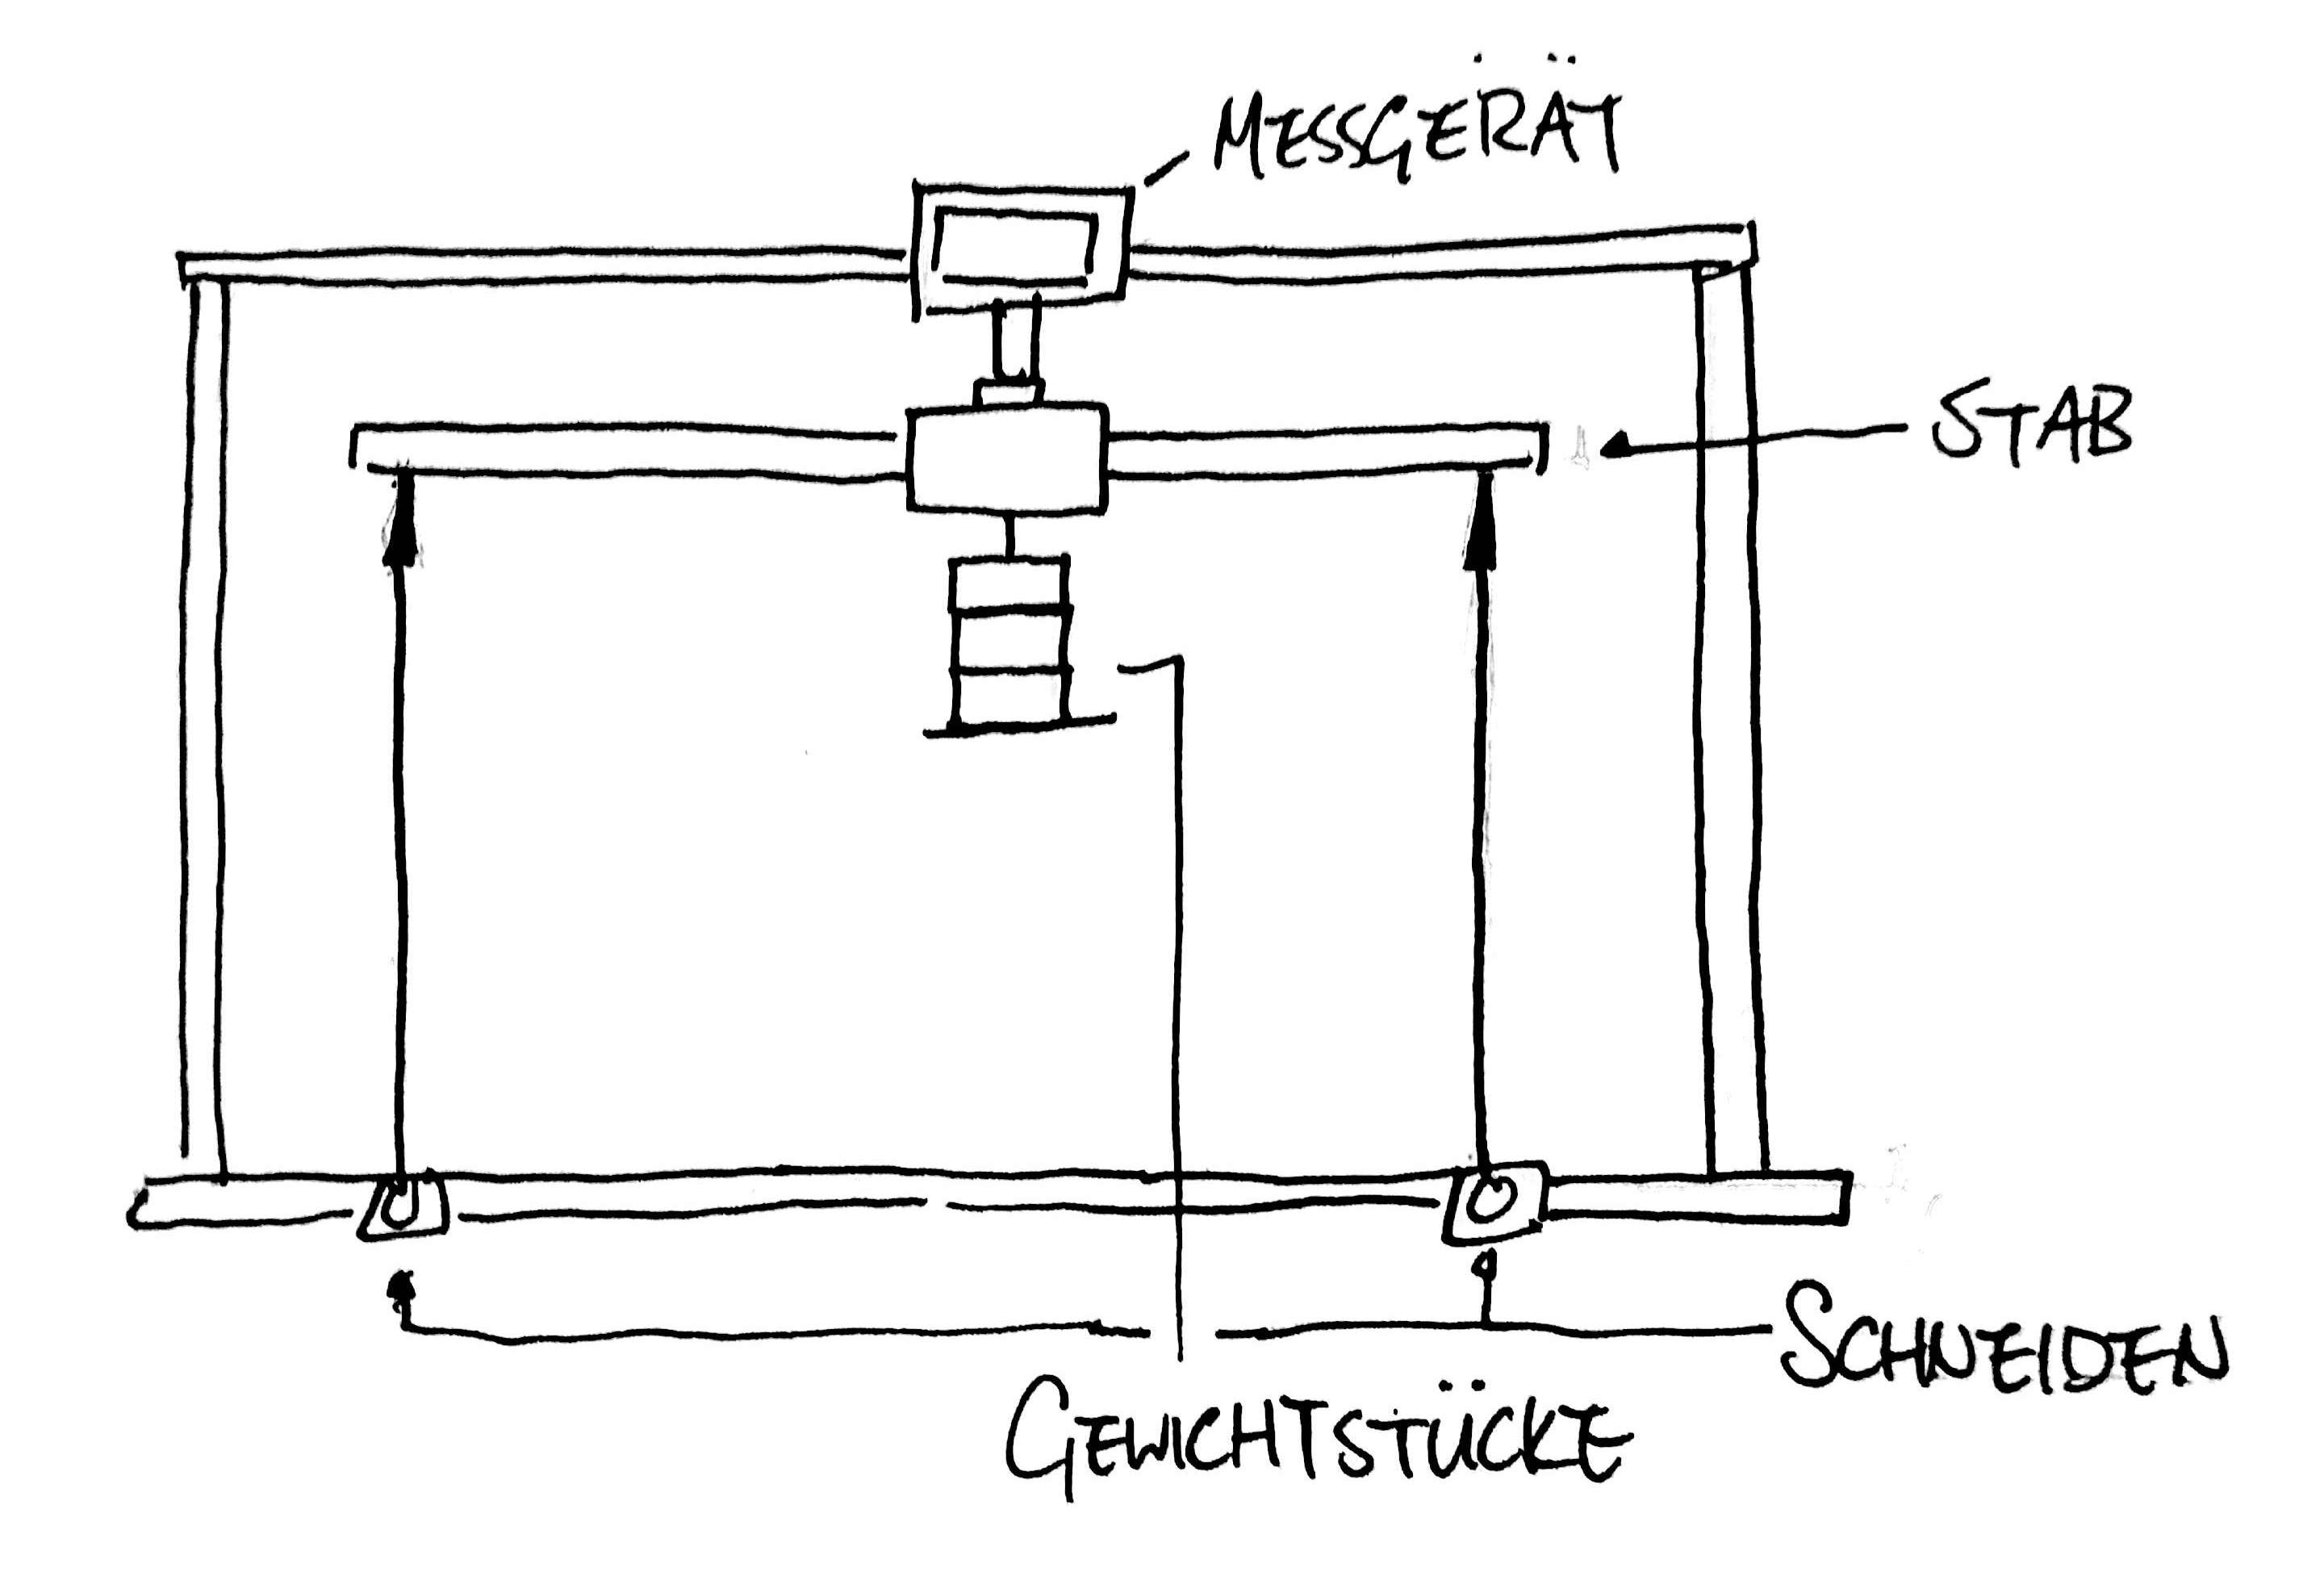
\includegraphics[width=\linewidth]{Abb1}
	\caption{Aufbau zum Versuch}
\end{figure}
Zum Versuch wurden zwei verschiebbare Schneiden, Stäbe aus mehreren Materialien, ein Maßband, Gewichtsstücke, eine Halterung für die Gewichtsstücke und ein Messgerät zur Bestimmung der Durchbiegung benutzt. 


\section{Versuchsdurchführung}
Zuerst wurden die Dimensionen der Stäbe (Breite und Höhe) gemessen. Jede Messung wurde fünfmal an anderen Stellen wiederholt. Danach wurden die einzelnen in dem Versuch verwendeten Gewichtsstücke gewogen und deren Massen aufgenommen. 

Für jede Messreihe wurde der Stab zuerst auf die zwei Schneiden gelegt. Es wurde mit dem Maßband sichergestellt, dass die Schneiden gleich entfernt von dem Mittelpunkt waren. Die Spitze des Messgeräts wurde auf die Halterung getan und das Gerät wurde geeicht. Es wurde dann eine relative große Masse auf die Halterung aufgehängt (In diesem Fall 6 große Gewichtsstücke). Der Abstand zwischen den Schneiden wurde dann geändert, sodass die angezeigte Durchbiegung zwischen 2 und 3mm lag. Danach wurden die Gewichtsstücke entfernt. 

Für die einzelnen Messungen wurden die Gewichtsstücke auf die Halterung aufgehängt. Für jede Gewichtsänderung wurde der auf dem Messgerät angezeigte Wert aufgenommen. Die Belastung wurde von kleineren zu größeren Werten variiert und wieder in umgekehrter Reihenfolge, um zwei Messwerte für jede Gewicht aufnehmen zu können. 

Dieser Prozesse wurde für unterschiedliche Materialien, Ausrichtungen des Stabes und Abstände zwischen den Schneiden wiederholt. 






\section{Auswertung und Fehleranalyse}
Die Durchschnittlichen Abmessungen der drei Stäbe und deren Unsicherheiten sind:

\begin{table} [h]
	\begin{tabular*}{0.99\textwidth}{@{\extracolsep{\fill}}c|cccccc}
		\toprule
		Material & Seite 1 & $u_\textrm{Seite 1}$ & Seite 2 & $u_\textrm{Seite 2}$  \\
		& mm & mm & mm & mm & \\
		\bottomrule
		Stahl & 5,916 & 0,005 & 9,910 & 0,007 \\
		Aluminium & 5,948 & 0,007 & 9,914 & 0,008 \\
		Messing & 5,914 & 0,005 & 9,902 & 0,004 \\
		\bottomrule
	\end{tabular*}
	\caption{Die Durchschnittlichen Abmessungen der Stäbe}
\end{table}

\begin{tcolorbox}[colback=white]
	\subsection{Rechenweg}
	Zur Berechnung der Mittelwerte wurde die folgende Formel verwendet:
	$$\bar{x} = \frac{1}{n} \sum_{i=1}^{n} x_i$$
	Für die Unsicherheiten wurden die Standardabweichung benutzt, nämlich:
	$$s_x = \sqrt{\frac{\sum_{i=1}^{n}(x_i-\bar{x})^2}{n-1}} $$
	
\end{tcolorbox}

Für jede Messreihe wurden die jeweiligen Mittelwerte in einer Graph aufgetragen (Siehe Abbildungen 1 bis 3). 

\begin{figure}[h]
	\centering
	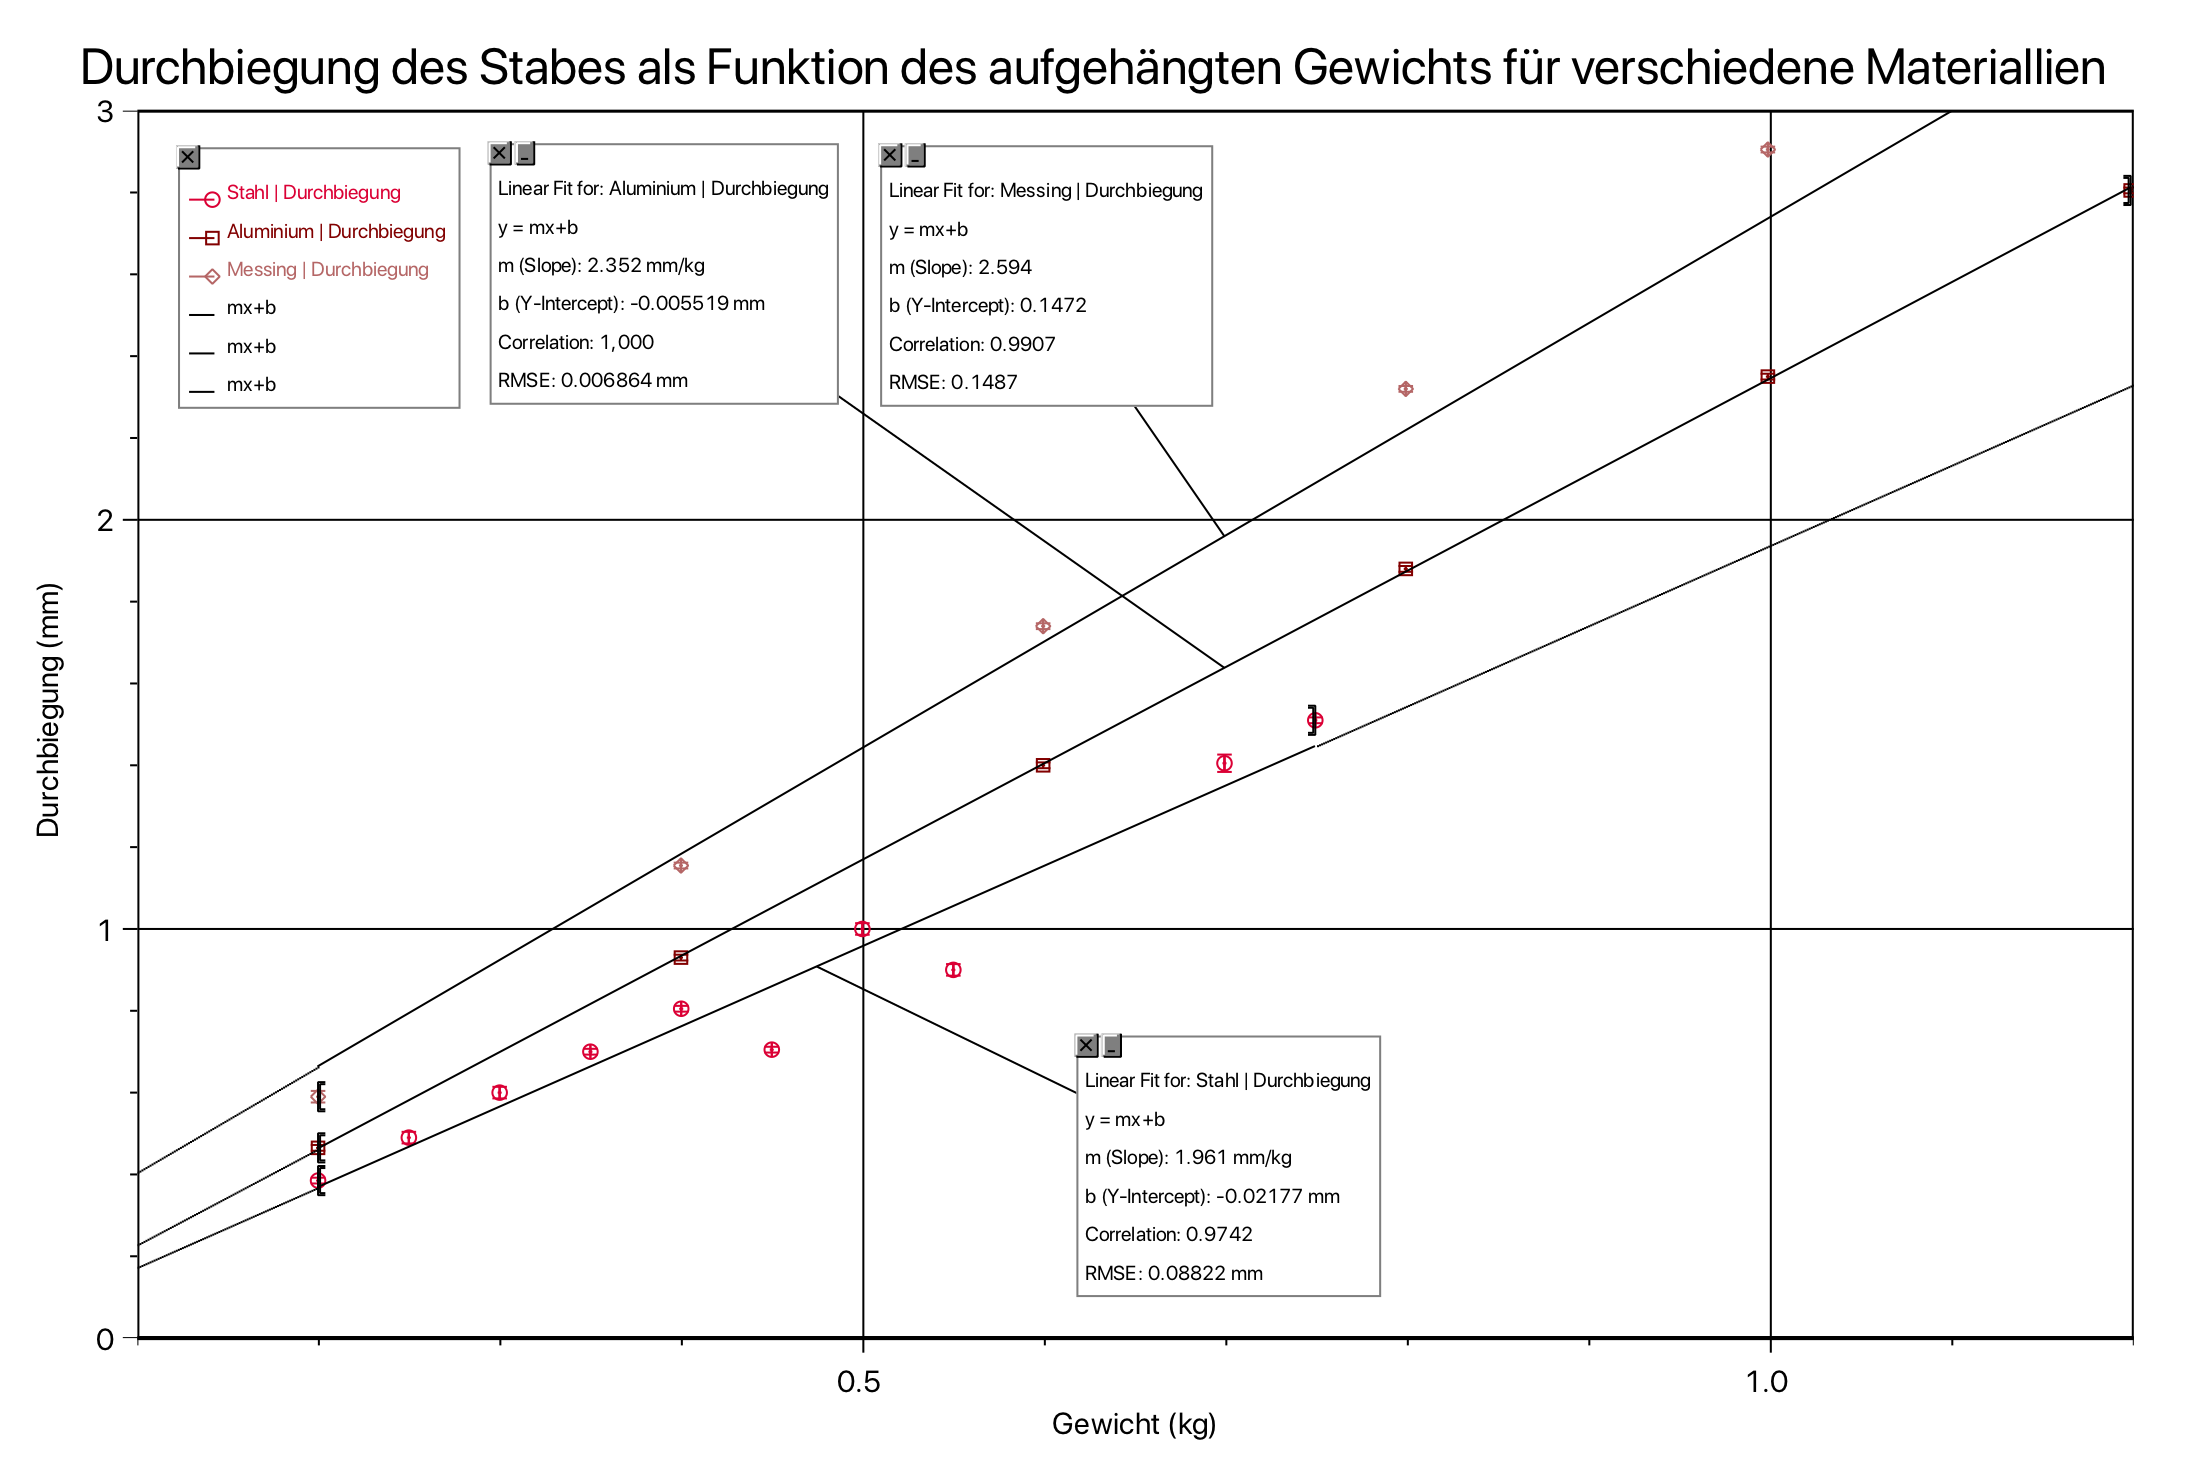
\includegraphics[width=\linewidth]{Abb2}
	\caption{Datenpunkte und Ausgleichsgeraden für verschiedene Materialien}
\end{figure}

\begin{figure}[h]
	\centering
	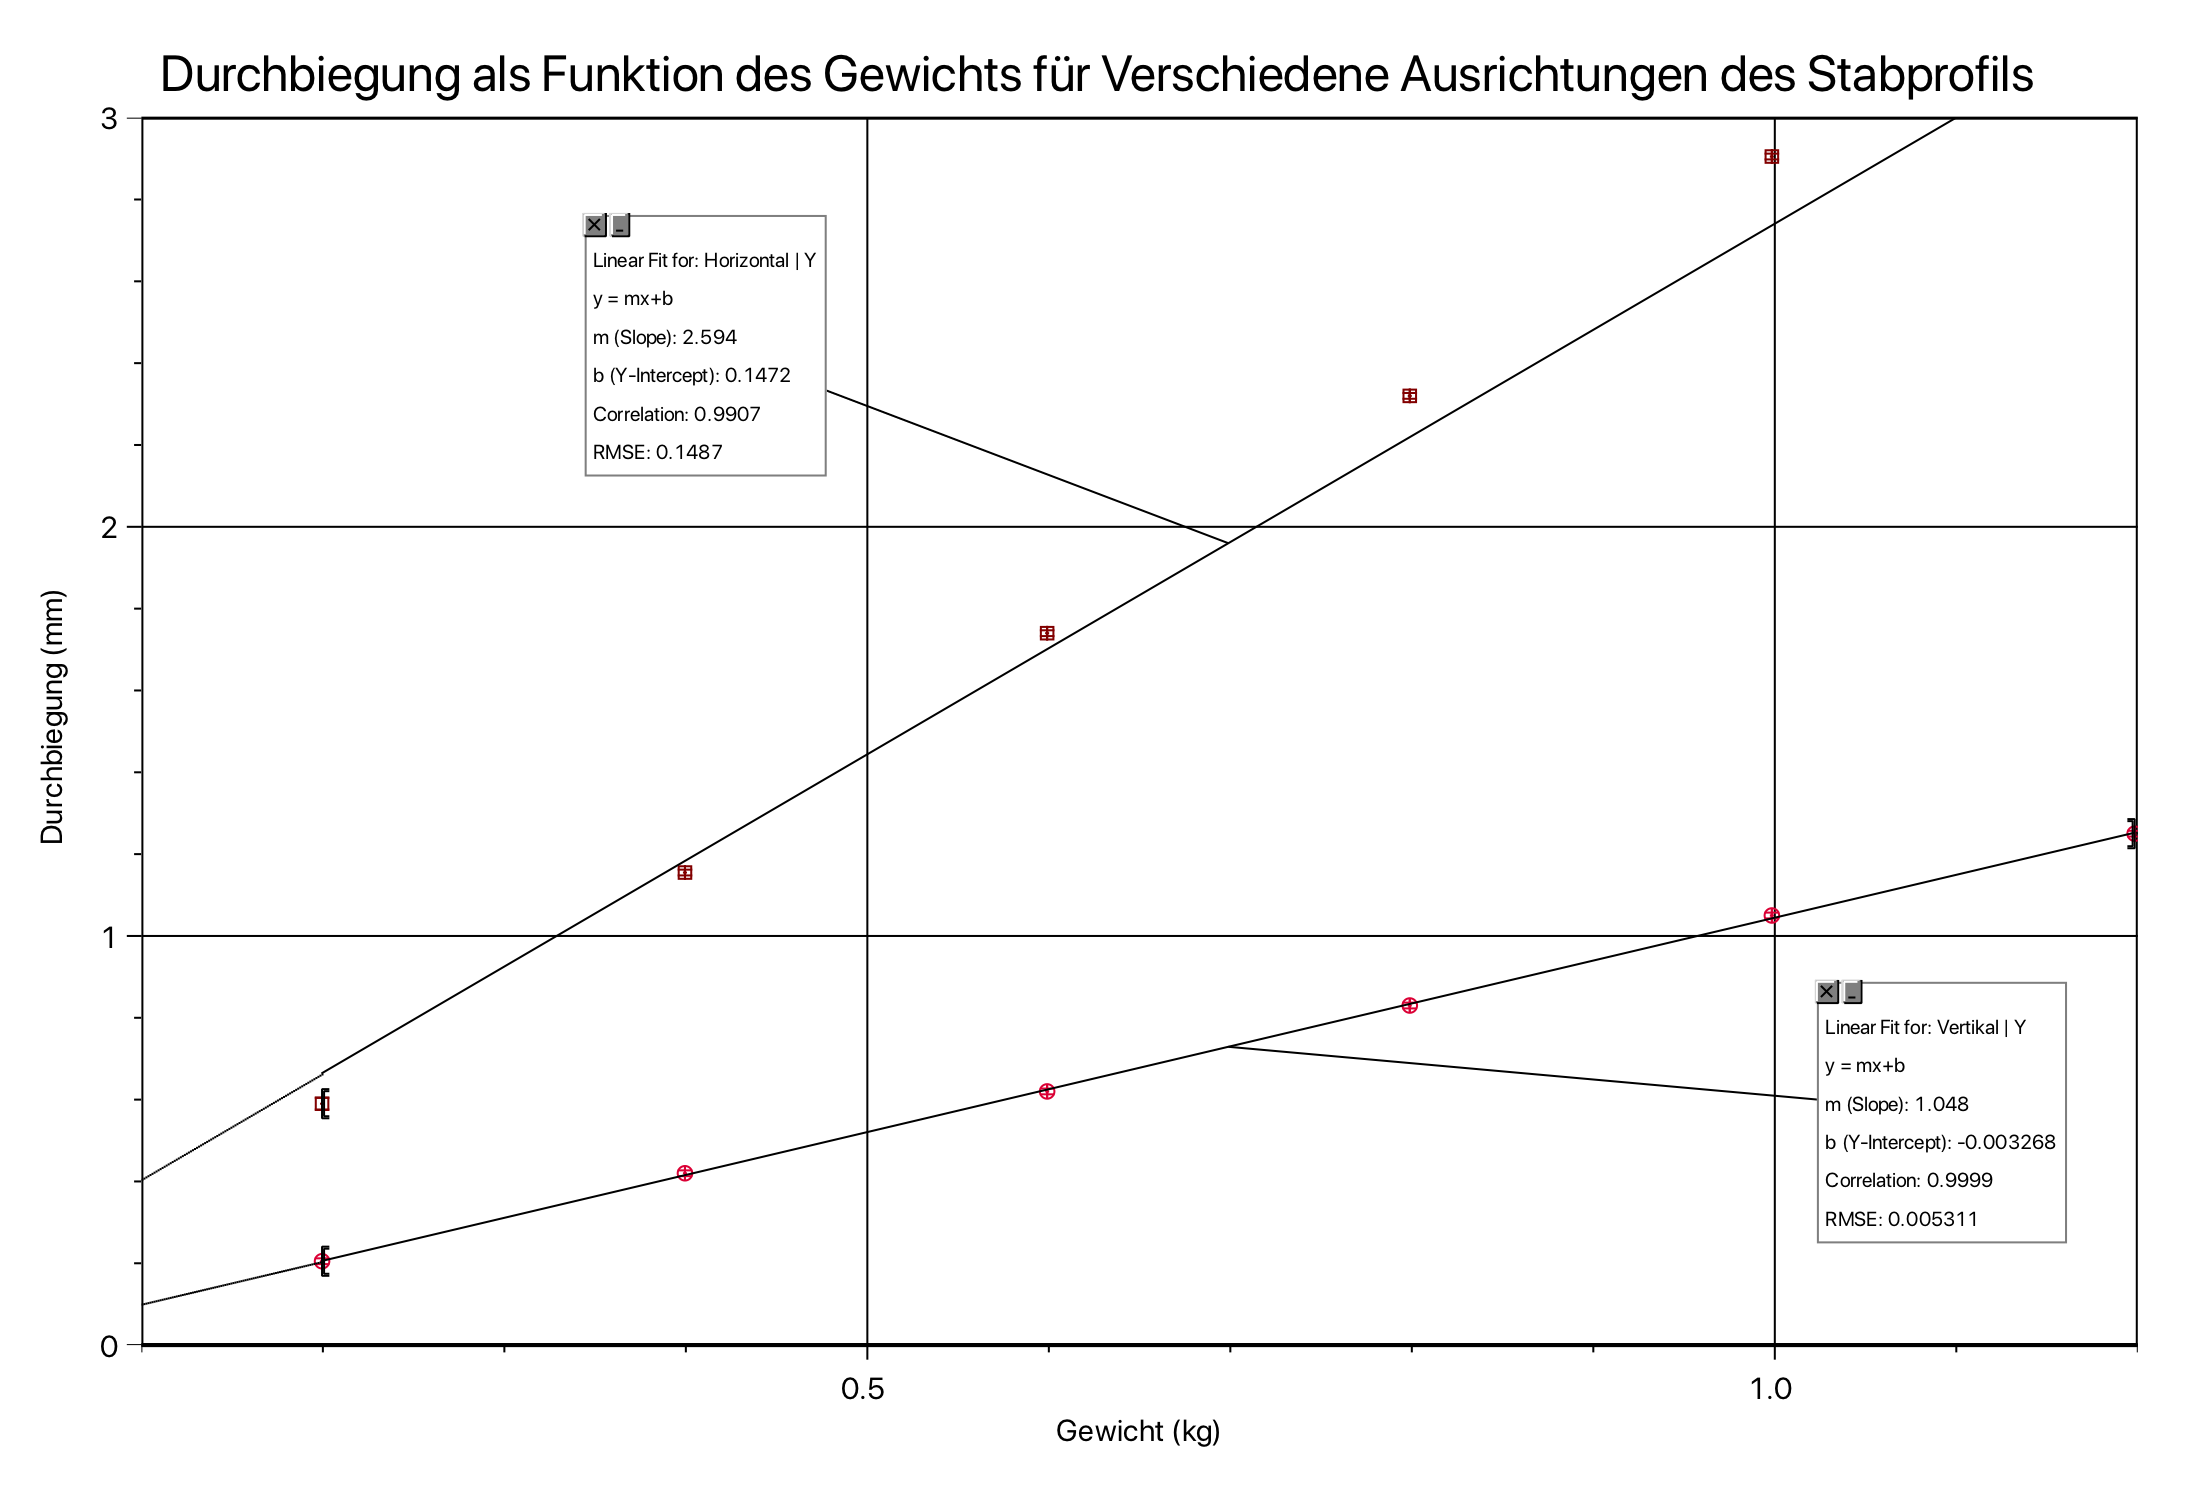
\includegraphics[width=\linewidth]{Abb3}
	\caption{Datenpunkte und Ausgleichsgeraden für unterschiedliche Ausrichtungen des Stabprofils}
\end{figure}

\begin{figure}[h]
	\centering
	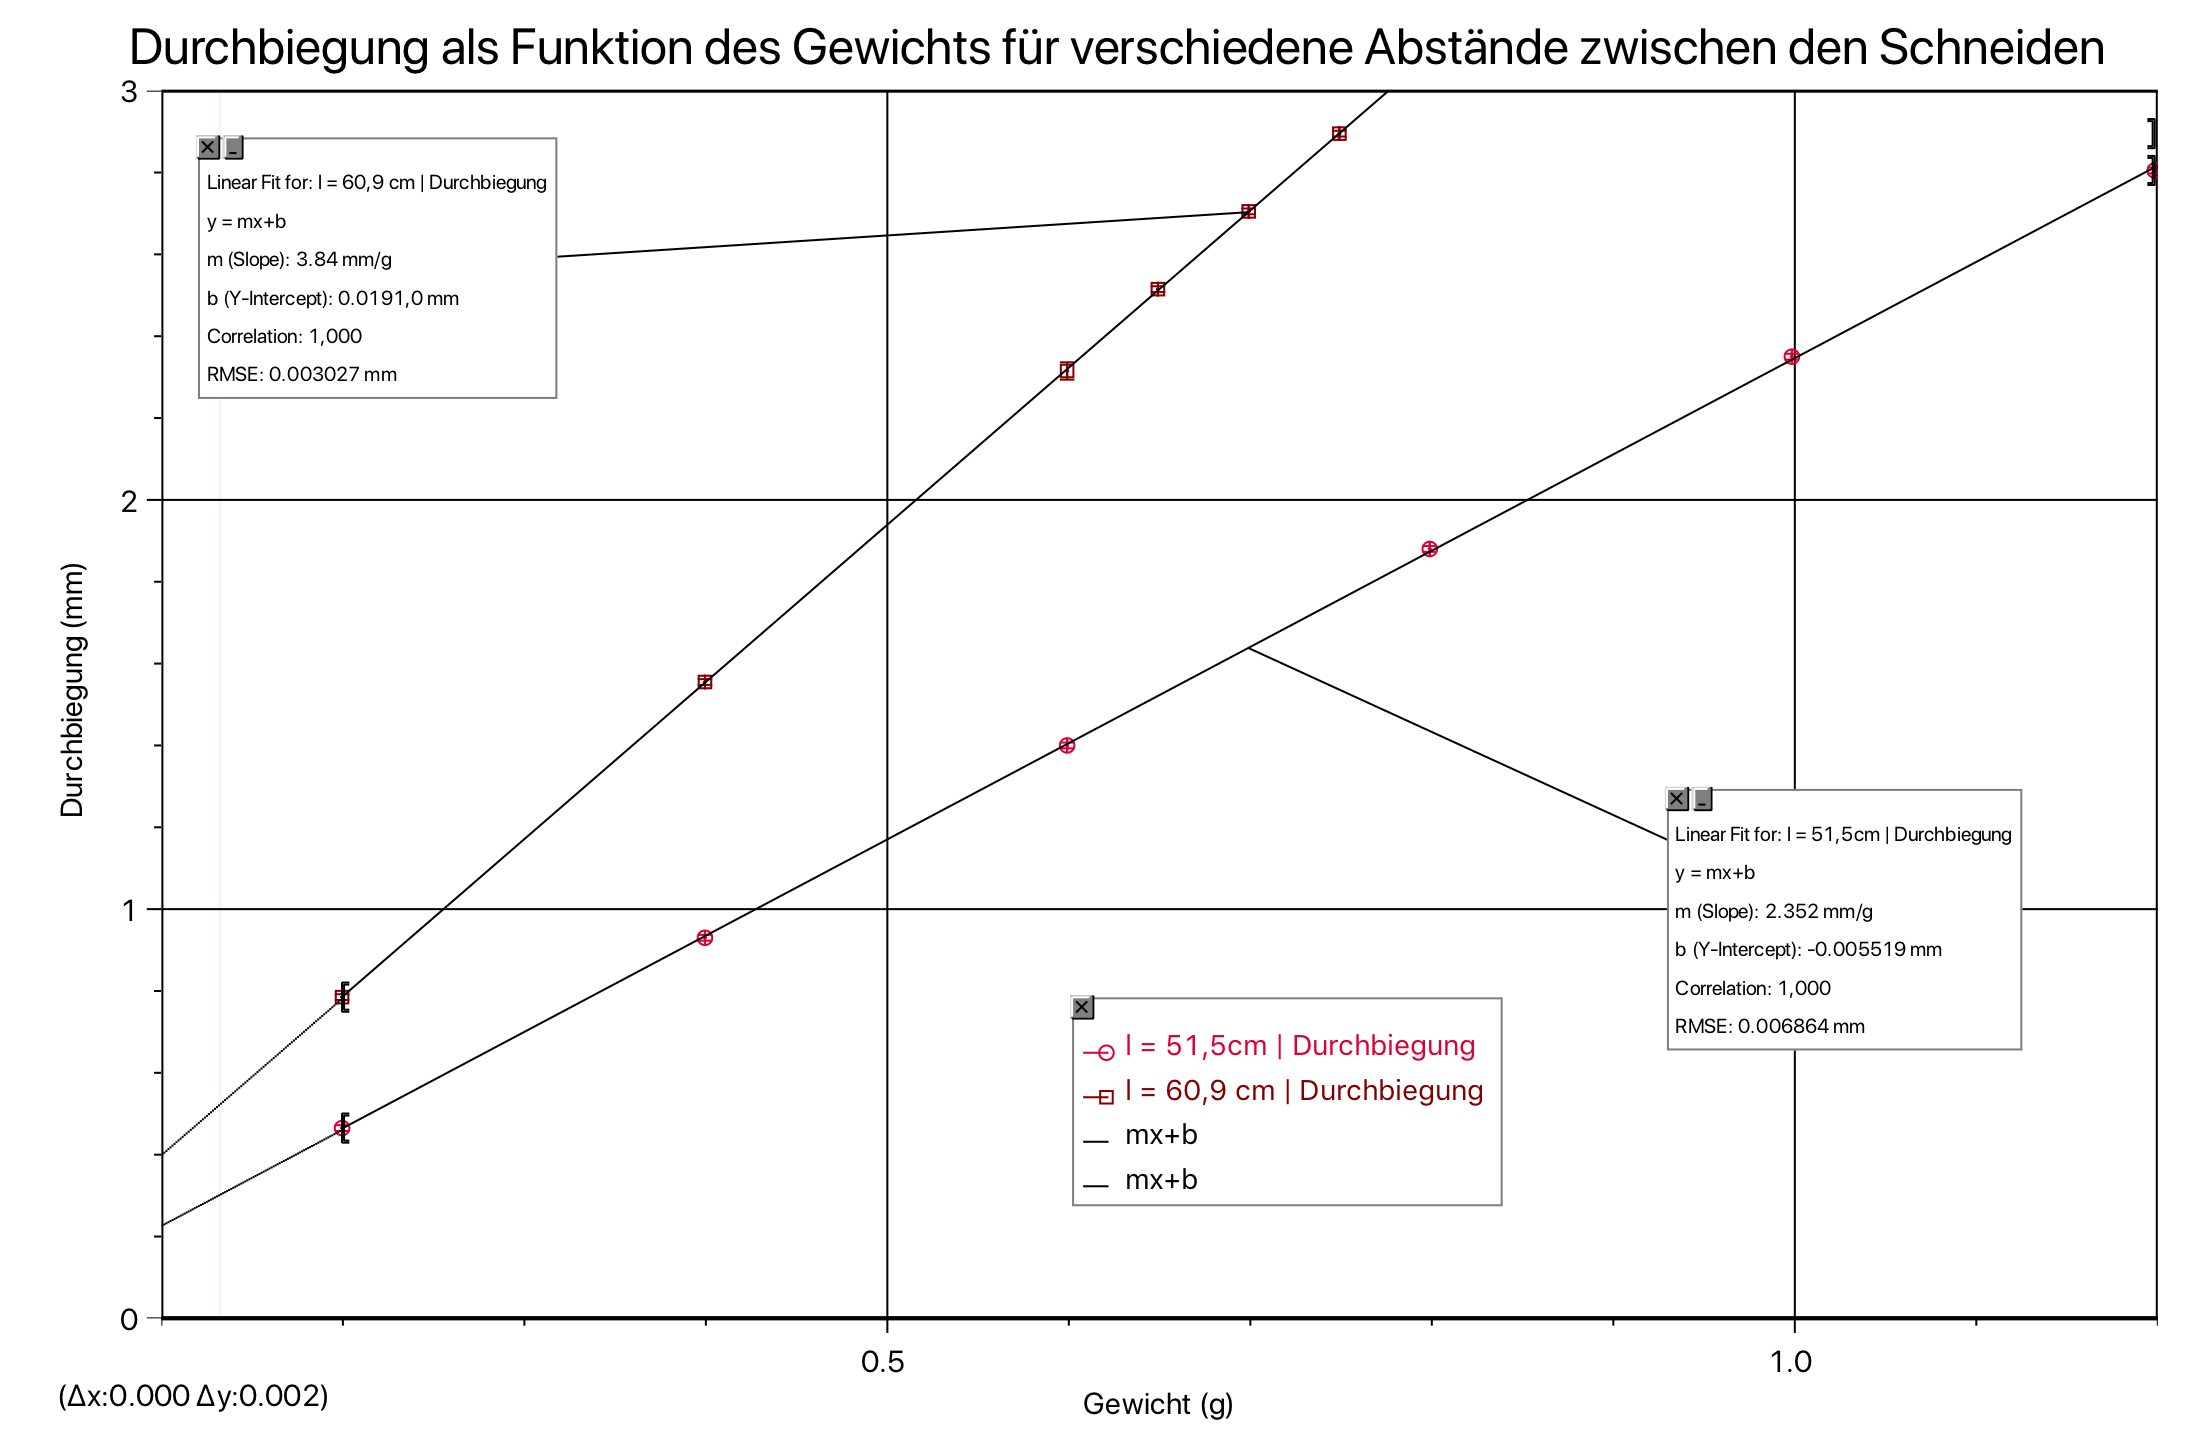
\includegraphics[width=\linewidth]{Abb4}
	\caption{Datenpunkte und Ausgleichsgeraden für verschiedene Abstände zwischen den Schneiden}
\end{figure}
\FloatBarrier

	Für die Unsicherheiten der einzelnen Punkte wurde die Standardunsicherheit wie oben benutzt, aber wenn es keine Abweichungen zwischen beiden Messwerten gab, wurde der Messfehler durch einen Faktor $\sqrt{n}$ geteilt. 

Mit einem Excel-Dokument wurde die lineare Regressionen und deren Unsicherheiten berechnet. Die linearen Zusammenhänge lassen sich in der Form: 
$$ s = a + bm $$ schreiben. Die einzelne Werte für $a$ und $b$ für jede Messreihe sind in Tabelle 1 bis 3 zu sehen (Achtung, dass in diesem Kontext $b$ nicht die Breite des Stabes ist). 

\begin{table} [h]
	\begin{tabular*}{0.99\textwidth}{@{\extracolsep{\fill}}c|cccccc}
		\toprule
		Material & $a$ & $u_a$ & $b$ & $u_b$  \\
		 & mm & mm & mm kg$^{-1}$ & mmkg$^{-1}$ & \\
		\bottomrule
		Stahl & -0,013 & 0,004 & 2,033 & 0,009 \\
		Aluminium & -0,006 & 0,006 & 2,352 & 0,008 \\
		Messing & 0,1 & 0,1 & 2,6 & 0,2 \\
		\bottomrule
	\end{tabular*}
	\caption{Werte für $a$ und $b$ und deren Unsicherheiten für verschiedene Materialien}
\end{table}

\begin{table} [h]
	\begin{tabular*}{0.99\textwidth}{@{\extracolsep{\fill}}c|cccccc}
		\toprule
		Ausrichtung & $a$ & $u_a$ & $b$ & $u_b$  \\
		& mm & mm & mm kg$^{-1}$ & mmkg$^{-1}$ & \\
		\bottomrule
		Horizontal & -0,006 & 0,006 & 2,352 & 0,008 \\
		Vertikal & -0,003 & 0,005 & 1,048 & 0,006 \\
		
		\bottomrule
	\end{tabular*}
	\caption{Werte für $a$ und $b$ und deren Unsicherheiten für unterschiedliche Ausrichtungen des Stabprofils (Messing)}
\end{table}

\begin{table} [h]
	\begin{tabular*}{0.99\textwidth}{@{\extracolsep{\fill}}c|cccc}
		\toprule
		Abstand & $a$ & $u_a$ & $b$ & $u_b$  \\
		cm & mm & mm & mm kg$^{-1}$ & mmkg $^{-1}$  \\
		\bottomrule
		51,5 & -0,006 & 0,006 & 2,352 & 0,008 \\
		60,9 & 0,019 & 0,004 & 3,840 & 0,006 \\
		
		\bottomrule
	\end{tabular*}
	\caption{Werte für $a$ und $b$ und deren Unsicherheiten für unterschiedliche Abstände zwischen den Schneiden (Aluminium)}
\end{table}
\FloatBarrier
Mit Formel (2) und $F = mg$ kann man leicht sehen, dass die Steigung $b$ dem Wert $\frac{1}{E}\frac{gl^3}{4h^3b}$ entspricht. Dadurch lässt sich der Wert von $E$ berechnen:
$$ E = \frac{gl^3}{4h^3bS}$$
In dieser Formel ist $S$ die Steigung, um Verwechslung mit dem Buchstabe für Breite zu vermeiden. Die berechneten Werte für $E$ und deren Unsicherheiten für die erste Messreihe sind:
$$E_\textrm{Stahl} = (21000 \pm 1000) \textrm{N/mm}^2$$
$$E_\textrm{Al} = (68300 \pm 500) \textrm{N/mm}^2 $$
$$E_\textrm{Messing} = (104000 \pm 8000) \textrm{N/mm}^2 $$
Für die zweite Messreihe:
$$E_\textrm{Messing-Vert} = (91600 \pm 700) \textrm{N/mm}^2 $$
und Für die dritte Messreihe:
$$E_\textrm{Al}' = (69000 \pm 1000) \textrm{N/mm}^2 $$

\begin{tcolorbox}[colback=white]
	\subsection{Rechenweg}
	Zur Berechnung der Unsicherheiten wurde die vereinfachte gauß'sche Fehlerfortpflanzung für Produkte und Quotienten benutzt:
	$$
	\left 
	\vert \frac{u_E}{E} \right \vert 
	 = \sqrt{(3\frac{u_l}{l})^2+(\frac{u_h}{h})^2+(3\frac{u_b}{b})^2+(\frac{u_S}{S})^2} $$
	
	
\end{tcolorbox}
\subsection{Biegsamkeit}
Die Einzelergebnisse für die Biegsamkeit, $\frac{ds}{dm} = S$, und deren Unsicherheiten sind in Abbildung (5) zu sehen:

\begin{figure}[h]
	\centering
	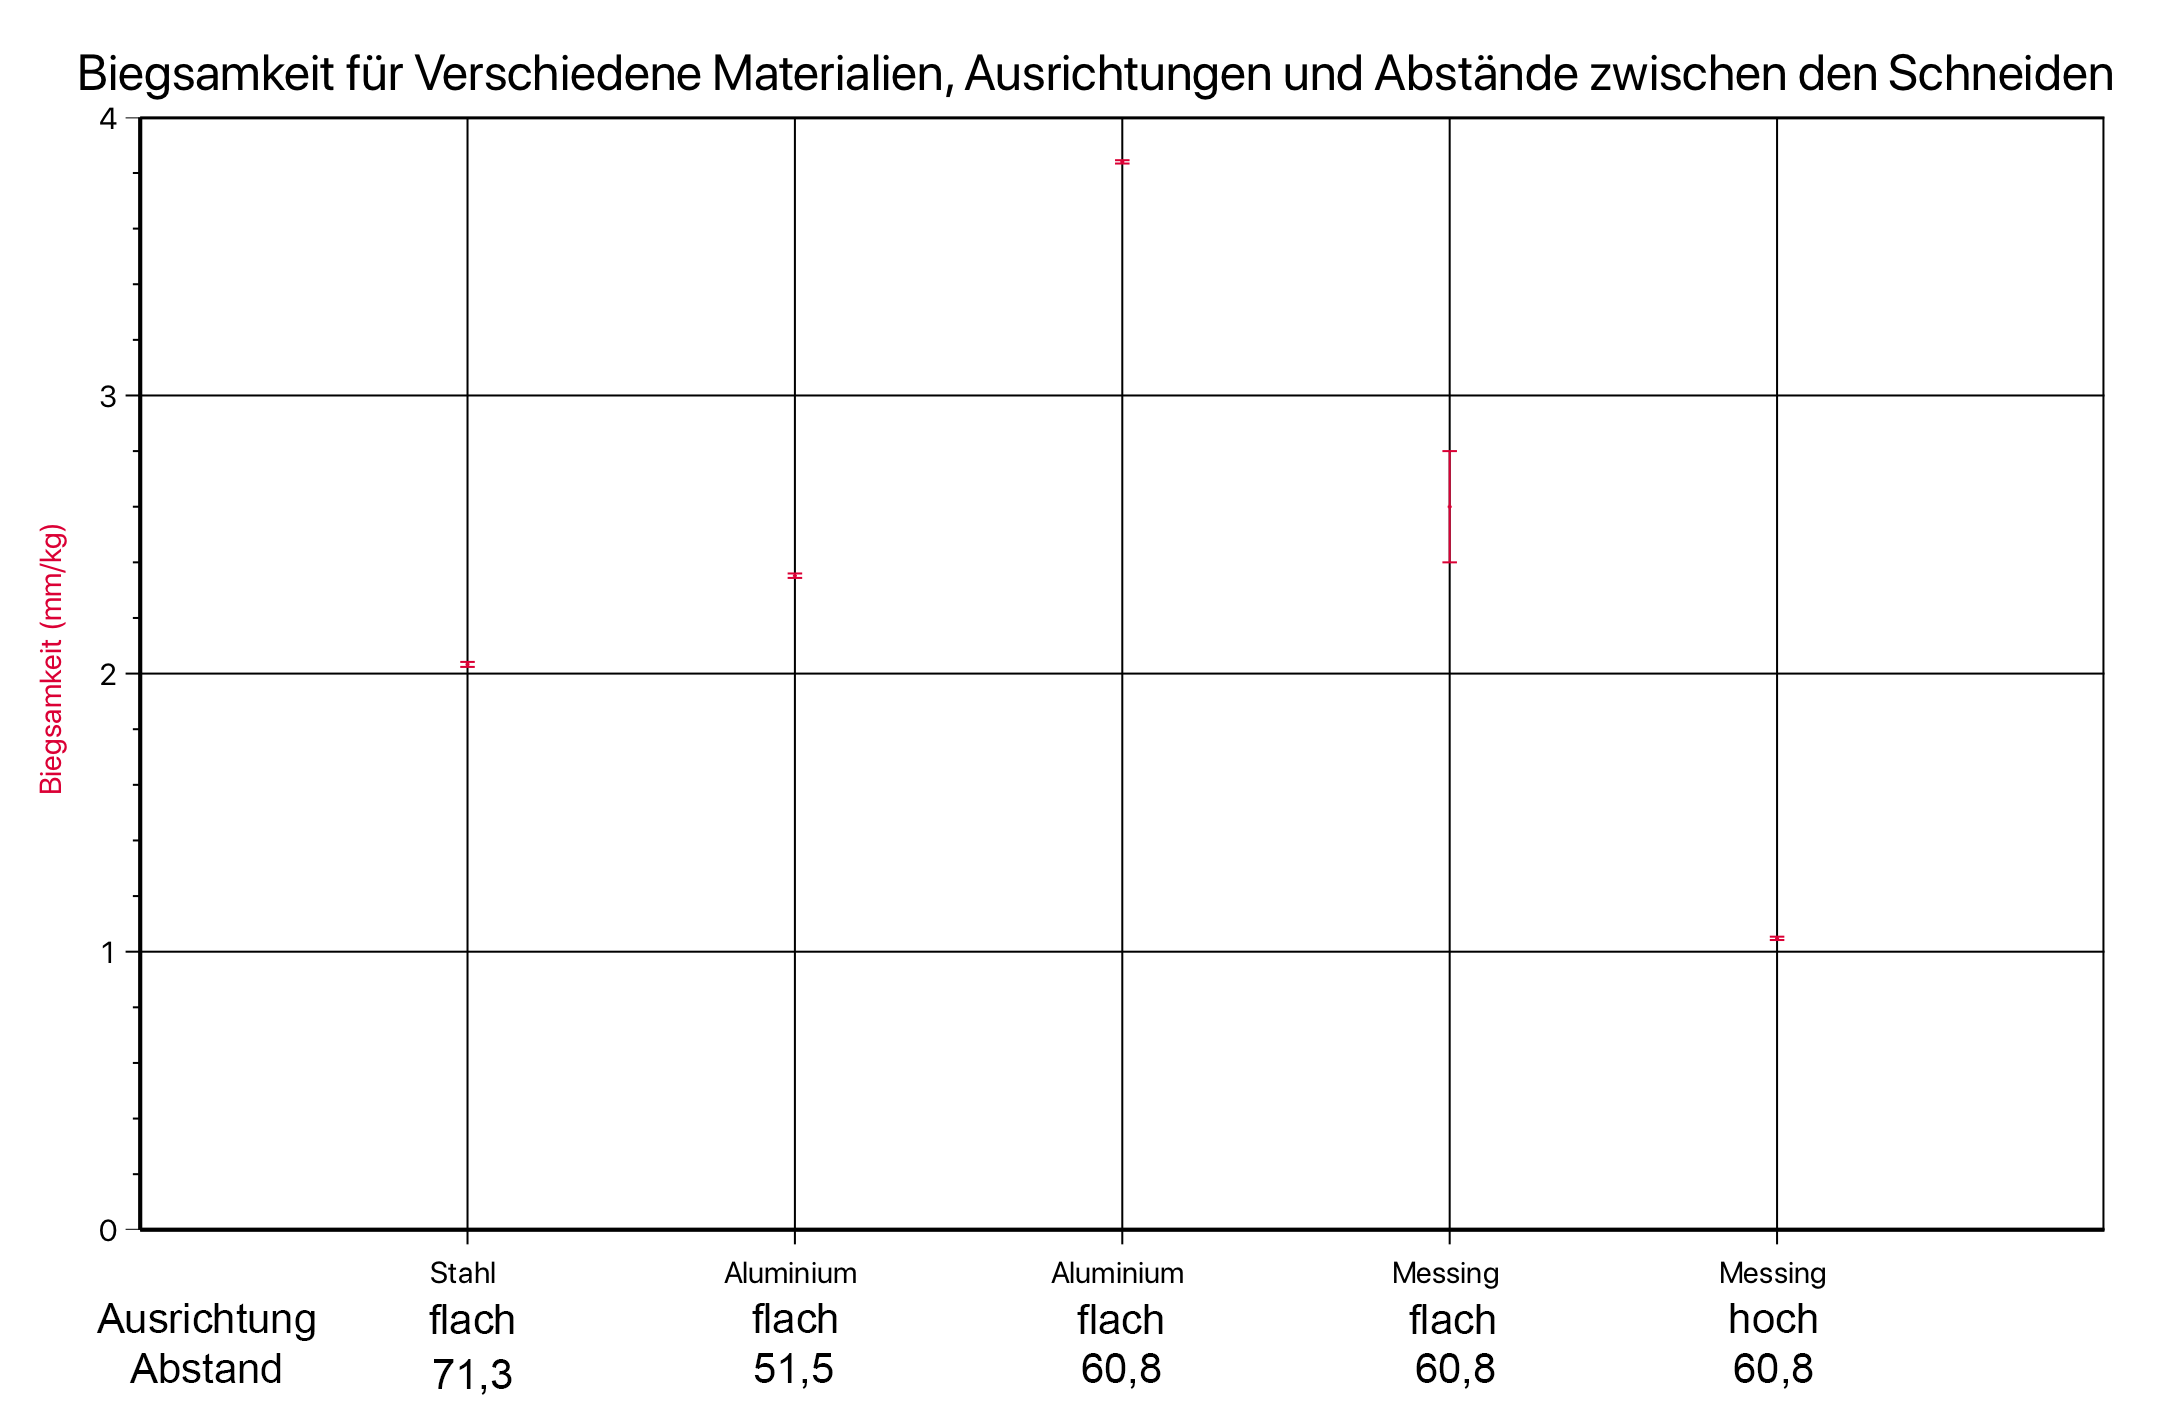
\includegraphics[width=\linewidth]{Abb5}
	\caption{Die gemessenen Biegsamkeit für jede Messreihe}
\end{figure}


\section{Diskussion der Ergebnisse}
Der berechnete Elastizitätsmodul von Stahl ist:
$$E_\textrm{Stahl} = (21000 \pm 1000)\textrm{N/mm}^2$$
und der von Aluminium für beide Messreihen:
$$E_\textrm{Al} = (68300 \pm 500)\textrm{N/mm}^2$$
$$E'_\textrm{Al} = (69000 \pm 1000)\textrm{N/mm}^2$$
und der von Messing für beide Messreihen:
$$E_\textrm{Messing} = (104000 \pm 8000)\textrm{N/mm}^2$$
$$E_\textrm{Messing-Vert} = (91600 \pm 700)\textrm{N/mm}^2$$

\subsection{Vergleich mit anderen Messmethoden und den Literaturwerten}
Um zu sehen, ob die beide Ergebnisse für den Elastizitätsmodul von Aluminium übereinstimmen, wurde ihre Differenz in Einheiten der kombinierten Standardunsicherheit berechnet, nämlich:
$$ t_\textrm{Al} = \frac{|E_\textrm{Al}-E'_\textrm{Al}|}{
\sqrt{u_{E'_\textrm{Al}}^2+u_{E'_\textrm{Al}}^2}}$$
$$ t \approx 0,62 $$
Da $t$ kleiner als 2 ist, sind beide Ergebnisse miteinander verträglich. Diese Verträglichkeit ist auch signifikant, da beide Unsicherheiten kleiner als 2\% der Werte selbst sind. 

Dasselbe Verfahren wurde auch für Messing durchgeführt.
$$ t_\textrm{Messing} \approx 1,515 $$
, was auch impliziert, dass die beiden Werte verträglich sind. Da $E_\textrm{Messing}$ eine relative große Unsicherheit hat (7\%), ist dieses Ergebnis aber von kleinerer Bedeutung. 

Den Versuchsanleitungen zufolge sind die Literaturwerte der Elastizitätsmodule:
$$E_\textrm{Al} = (69 ... 72,5) \textrm{N/mm}^2$$
$$E_\textrm{Stahl} = (195 ... 210) \textrm{N/mm}^2$$
$$E_\textrm{Messing} = (90 ... 95) \textrm{N/mm}^2$$
Es kann sofort gesehen werden, dass $E_\textrm{Stahl}$, $E'_\textrm{Al}$ und $E_\textrm{Messing-Vert}$ innerhalb der Rahmen der Literaturwerten liegen. Deswegen sind diese Ergebnisse und die Literaturwerte miteinander verträglich. 

Falls der gemessene Wert außerhalb der Rahmen des Literaturwertes lag, wurde die Differenz in Einheiten ihrer Standardunsicherheiten berechnet, um zu sehen, ob der gemessene Wert und der Literaturwert miteinander verträglich sind. 
$$t_{E_\textrm{Al}} = 1,4$$
$$t_{E_\textrm{Messing}} = 1,125$$
Da diese Werte kleiner als 2 sind, sind alle gemessenen Werte und die Literaturwerte miteinander verträglich. 
\subsection{Systematische und Statistische Fehler und Verbesserungsvorschläge}
Ein statistischer Fehler war es, das die Schneiden nicht ganz stabil waren. Deswegen war es schwierig, den wirklichen Abstand zwischen den Schneiden akkurat zu messen, ohne sie zu kippen. Dieses Problem lässt sich dadurch lösen, indem man kürzere Schneiden benutzt, die nicht so viel wackeln können. 

Ein möglicher systematischer Fehler ist die elastische Hysterese, wobei bei Spannung und Entspannung unterschiedliche Dehnungen gemessen wird, obwohl das Objekt mit gleicher Kraft gespannt wird. Deswegen ist es möglich, dass dieselbe Durchbiegung nicht gemessen wird (bei der Entlastung nach den ersten Messungen), obwohl der Stab genau wie vorher belastet ist. Es wurde aber keine messbare Hysterese mit dem gegebenen Messgerät gemessen und deshalb wurde der Effekt von der elastischen Hysterese bei der Auswertung vernachlässigt. 




\section{Literatur}
,,Versuchsanleitung zum Physiklabor für Anfänger*innen.'' Albert-Ludwigs-Universität Freiburg. 
	
\section{Anhang}
Siehe Zusatzblatt
	
	
	
\end{document}